\documentclass[12pt, a4paper]{article}

% Packages
\usepackage[utf8]{inputenc}
\usepackage[T1]{fontenc}
\usepackage{times}
\usepackage[margin=1in]{geometry}
\usepackage{graphicx}
\usepackage{hyperref}
\usepackage{setspace}
\usepackage{titlesec}
\usepackage{parskip}
\usepackage{caption}
\usepackage{float}
\usepackage{fancyhdr}
\usepackage{booktabs}
\usepackage{amsmath}

% Formatting
\onehalfspacing
\titleformat{\section}{\large\bfseries}{\thesection.}{0.5em}{}
\titleformat{\subsection}{\normalsize\bfseries}{\thesubsection}{0.5em}{}
\hypersetup{
    colorlinks=true,
    linkcolor=black,
    urlcolor=blue,
    citecolor=black
}

% Header and Footer
\pagestyle{fancy}
\fancyhf{}
\fancyhead[L]{\small CS432 Database Project -- Module A}
\fancyhead[R]{\small B+ Tree DBMS Report}
\fancyfoot[C]{\thepage}
\renewcommand{\headrulewidth}{0.4pt}
\renewcommand{\footrulewidth}{0pt}

\begin{document}

% ==================== COVER PAGE ====================
\begin{titlepage}
\thispagestyle{empty}

% Top header line
\noindent{\small CS432 -- Assignment 2} \hfill {\small March 21, 2026}

\vspace{1pt}
\noindent\rule{\textwidth}{0.8pt}

\begin{center}

\vspace{0.8cm}

{\large \textbf{SubTask 6 Report}}

\vspace{1.2cm}

% Logo

\includegraphics[width=0.22\textwidth]{iitgn-logo.png}

\vspace{1.2cm}

{\normalsize \textbf{CS432 Database Systems}}\\[10pt]
{\small INDIAN INSTITUTE OF TECHNOLOGY GANDHINAGAR}\\[2pt]
{\small Palaj, Gandhinagar -- 382355}

\vspace{0.5cm}
\noindent\rule{0.8\textwidth}{0.8pt}

\vspace{0.5cm}

{\LARGE \textbf{B+ Tree-Based DBMS for Campus Trading}}

\vspace{0.1cm}

{\large Implementation, Benchmarking and Visual Analysis}

\vspace{0.5cm}

\noindent\rule{0.4\textwidth}{0.4pt}

\vspace{0.4cm}

{\normalsize \textbf{Submitted by}}

\vspace{0.4cm}

{\normalsize \textbf{Team 8}}\\[4pt]
{\normalsize Bhavik Patel, Hitesh Kumar, Jinil Patel, Pranav Patil, Sibtain}

\end{center}

\end{titlepage}

\tableofcontents
\newpage

\section{Introduction}
\subsection{Problem Addressed}
The Campus Trading application requires efficient data access over continuously growing datasets, including listings, members, offers, and transactions. Typical workloads include exact-key lookup (for example, by listing ID) and range-based filtering (for example, price windows). A linear baseline requires \(O(n)\) scans, which becomes a bottleneck as the dataset grows. In practical terms, this directly affects user-facing tasks such as filtering listings by budget, loading searchable catalog views, and retrieving record details under frequent concurrent interactions.

From a systems perspective, the core challenge is to maintain \textbf{query responsiveness} while data volume grows. Without a structured index, performance degradation becomes unavoidable as every query tends toward full traversal. Therefore, an index design that supports both point and range access patterns is essential for this project context.

\subsection{Proposed Solution}
We implemented a B+ Tree-based indexing layer to provide stable and scalable DBMS-style performance. Under this design, point operations such as search, insert, update, and delete run in \(O(\log n)\), while range operations run in \(O(\log n + k)\). The linked-leaf structure supports ordered traversal directly, and balancing is preserved through split, borrow, and merge procedures during updates.

The proposed architecture is intentionally aligned with database indexing principles: internal nodes are used for routing only, while leaves hold data records in sorted order. This separation improves structural clarity, simplifies traversal logic, and enables \textbf{efficient range scans} with predictable asymptotic behavior.

\section{Implementation}
\subsection{Code Structure}
Key files used in Module A are listed below for clarity:
\begin{itemize}
    \item \texttt{database/node.py}: defines \texttt{Node}, \texttt{LeafNode}, and \texttt{InternalNode}.
    \item \texttt{database/bplustree.py}: implements search/insert/delete/update/range query and visualization.
    \item \texttt{database/table.py}: schema-aware table wrapper on top of B+ Tree.
    \item \texttt{database/db\_manager.py}: creates logical databases and manages tables.
    \item \texttt{database/benchmark.py}: compares B+ Tree vs brute-force baseline.
\end{itemize}

From an implementation perspective, the system is organized as a layered pipeline: node primitives define structural invariants, the B+ Tree layer enforces these invariants under updates, and the table/manager layers expose database-style APIs for CRUD and range filtering.

This layered approach also improves maintainability. The node layer encapsulates low-level invariants, the tree layer manages balancing semantics, and the table/manager layer maps these capabilities to application-facing data operations.

\subsection{Node Layer (\texttt{node.py})}
\textbf{Node class:} stores shared metadata such as \texttt{keys}, \texttt{parent}, and order-derived constraints:
\begin{itemize}
    \item \texttt{max\_keys()} returns \(m-1\),
    \item \texttt{min\_keys()} returns \(\lceil m/2 \rceil - 1\),
    \item \texttt{is\_full()} and \texttt{is\_underflow()} enforce occupancy rules.
\end{itemize}

\textbf{LeafNode:}
\begin{itemize}
    \item stores actual records in aligned \texttt{keys} and \texttt{values},
    \item maintains \texttt{next} and \texttt{prev} pointers for sequential scans,
    \item provides \texttt{insert\_at}, \texttt{remove\_at}, \texttt{get\_value}, \texttt{set\_value} used by B+ Tree operations.
\end{itemize}

\textbf{InternalNode:}
\begin{itemize}
    \item stores separator keys and child pointers,
    \item uses \texttt{find\_child\_index(key)} (binary-search style routing) to select the correct subtree,
    \item powers root-to-leaf navigation via \texttt{get\_child\_for\_key}.
\end{itemize}

Algorithmically, this layer provides two guarantees on which the tree layer depends: \textit{(i)} local occupancy constraints for each node, and \textit{(ii)} deterministic routing to exactly one child for any search key.

\subsection{B+ Tree Layer (\texttt{bplustree.py})}
\subsubsection{Algorithmic View of Core Operations}
\textbf{Search Algorithm}
\begin{enumerate}
    \item Start from root.
    \item Repeatedly route through internal separators until a leaf is reached.
    \item Resolve key in the leaf array.
\end{enumerate}

\textbf{Insert Algorithm}
\begin{enumerate}
    \item Route to target leaf.
    \item If key exists, overwrite value (upsert behavior).
    \item Else insert in sorted order.
    \item If node overflows, split node and propagate separator upward.
    \item If propagation reaches root overflow, create a new root.
\end{enumerate}

\textbf{Delete Algorithm}
\begin{enumerate}
    \item Route to target leaf and remove key.
    \item If node underflows, first try redistribution (borrow from siblings).
    \item If redistribution fails, merge with sibling and remove parent separator.
    \item Repeat upward while a parent violates occupancy constraints.
\end{enumerate}

Together, these procedures guarantee that the tree remains \textbf{balanced}, all leaves remain at the same depth, and key ordering is preserved after each update workload.

\subsubsection{Focused Functions: \texttt{update} and \texttt{range\_query}}
\textbf{Update (abstract flow)}
\begin{enumerate}
    \item Locate target leaf using the same routing path as search.
    \item Attempt in-place replacement of the value for the matching key.
    \item Return success/failure flag without changing structure.
\end{enumerate}

\textbf{Range Query (abstract flow)}
\begin{enumerate}
    \item Route to first leaf that may contain the lower bound.
    \item Traverse leaf linked-list left-to-right.
    \item Emit entries while keys are within \([start, end]\).
    \item Stop immediately once key exceeds upper bound.
\end{enumerate}

This two-phase range strategy (single logarithmic seek + sequential leaf scan) is the primary reason the index performs well for budget-window filtering in Campus Trading.

\subsubsection{Visualization Methods (\texttt{visualize\_tree} family)}
The visualization pipeline in \texttt{bplustree.py} combines:
\begin{itemize}
    \item \texttt{visualize\_tree}: creates graph object and orchestrates rendering,
    \item \texttt{\_add\_nodes}: draws leaf/internal node labels,
    \item \texttt{\_add\_edges}: draws parent-child edges,
    \item \texttt{\_add\_leaf\_links}: overlays dashed links for leaf-level ordering.
\end{itemize}
This makes structural properties visually verifiable during testing.

\subsection{Complexity Summary}
\begin{table}[H]
\centering
\caption{Time Complexity of Main Operations}
\begin{tabular}{@{}ll@{}}
\toprule
Operation & Complexity \\
\midrule
\texttt{search(key)} & \(O(\log n)\) \\
\texttt{insert(key, value)} & \(O(\log n)\) \\
\texttt{delete(key)} & \(O(\log n)\) \\
\texttt{update(key, value)} & \(O(\log n)\) \\
\texttt{range\_query(start, end)} & \(O(\log n + k)\) \\
\texttt{get\_all()} & \(O(n)\) \\
\bottomrule
\end{tabular}
\end{table}

The complexity profile confirms the intended design objective: operations scale logarithmically in tree size, while sequential extraction tasks remain linear in output size. This is especially appropriate for marketplace-style filtering and retrieval patterns.

\section{Performance Analysis}
\subsection{Benchmark Setup}
The benchmark compares B+ Tree and \texttt{BruteForceDB} for insertion, search, range query, and deletion across increasing dataset sizes.

Evaluation protocol used in the notebook:
\begin{enumerate}
    \item Generate reproducible random key-value datasets for each size.
    \item \textbf{Insert evaluation:} measure total insertion workload for both structures from an empty state.
    \item \textbf{Search evaluation:} sample approximately 10\% of inserted keys and measure point-lookup time.
    \item \textbf{Range evaluation:} execute multiple random intervals and measure total range-query workload.
    \item \textbf{Delete evaluation:} rebuild structures, delete a sampled fraction of keys, and measure total deletion workload.
    \item Repeat over all configured sizes and store operation-wise curves.
\end{enumerate}

All timings are collected in Python using high-resolution wall-clock timers and then plotted operation-wise for direct trend comparison.

To ensure a fair comparison, both structures receive equivalent datasets and equivalent operation counts per benchmark stage. For delete benchmarks, structures are reconstructed from the same seed-generated dataset before timing begins, preventing state carry-over effects from earlier measurements.

\subsection{Benchmark Findings}
The observed trends are consistent with theoretical complexity and remain stable across tested scales. Search shows the clearest widening performance gap as \(n\) increases, matching \(O(\log n)\) behavior for B+ Tree versus \(O(n)\) behavior for brute-force search. Range query performance also improves substantially because the B+ Tree performs a single logarithmic seek and then scans linked leaves sequentially. Insert and delete remain scalable despite occasional split/merge overhead, and this overhead does not alter asymptotic behavior.

Overall, the benchmark results support the key claim of this report: the B+ Tree index provides \textbf{better scalability} and \textbf{more predictable latency growth} than a linear baseline, particularly for high-volume lookup and filtering workloads.

\begin{figure}[H]
    \centering
    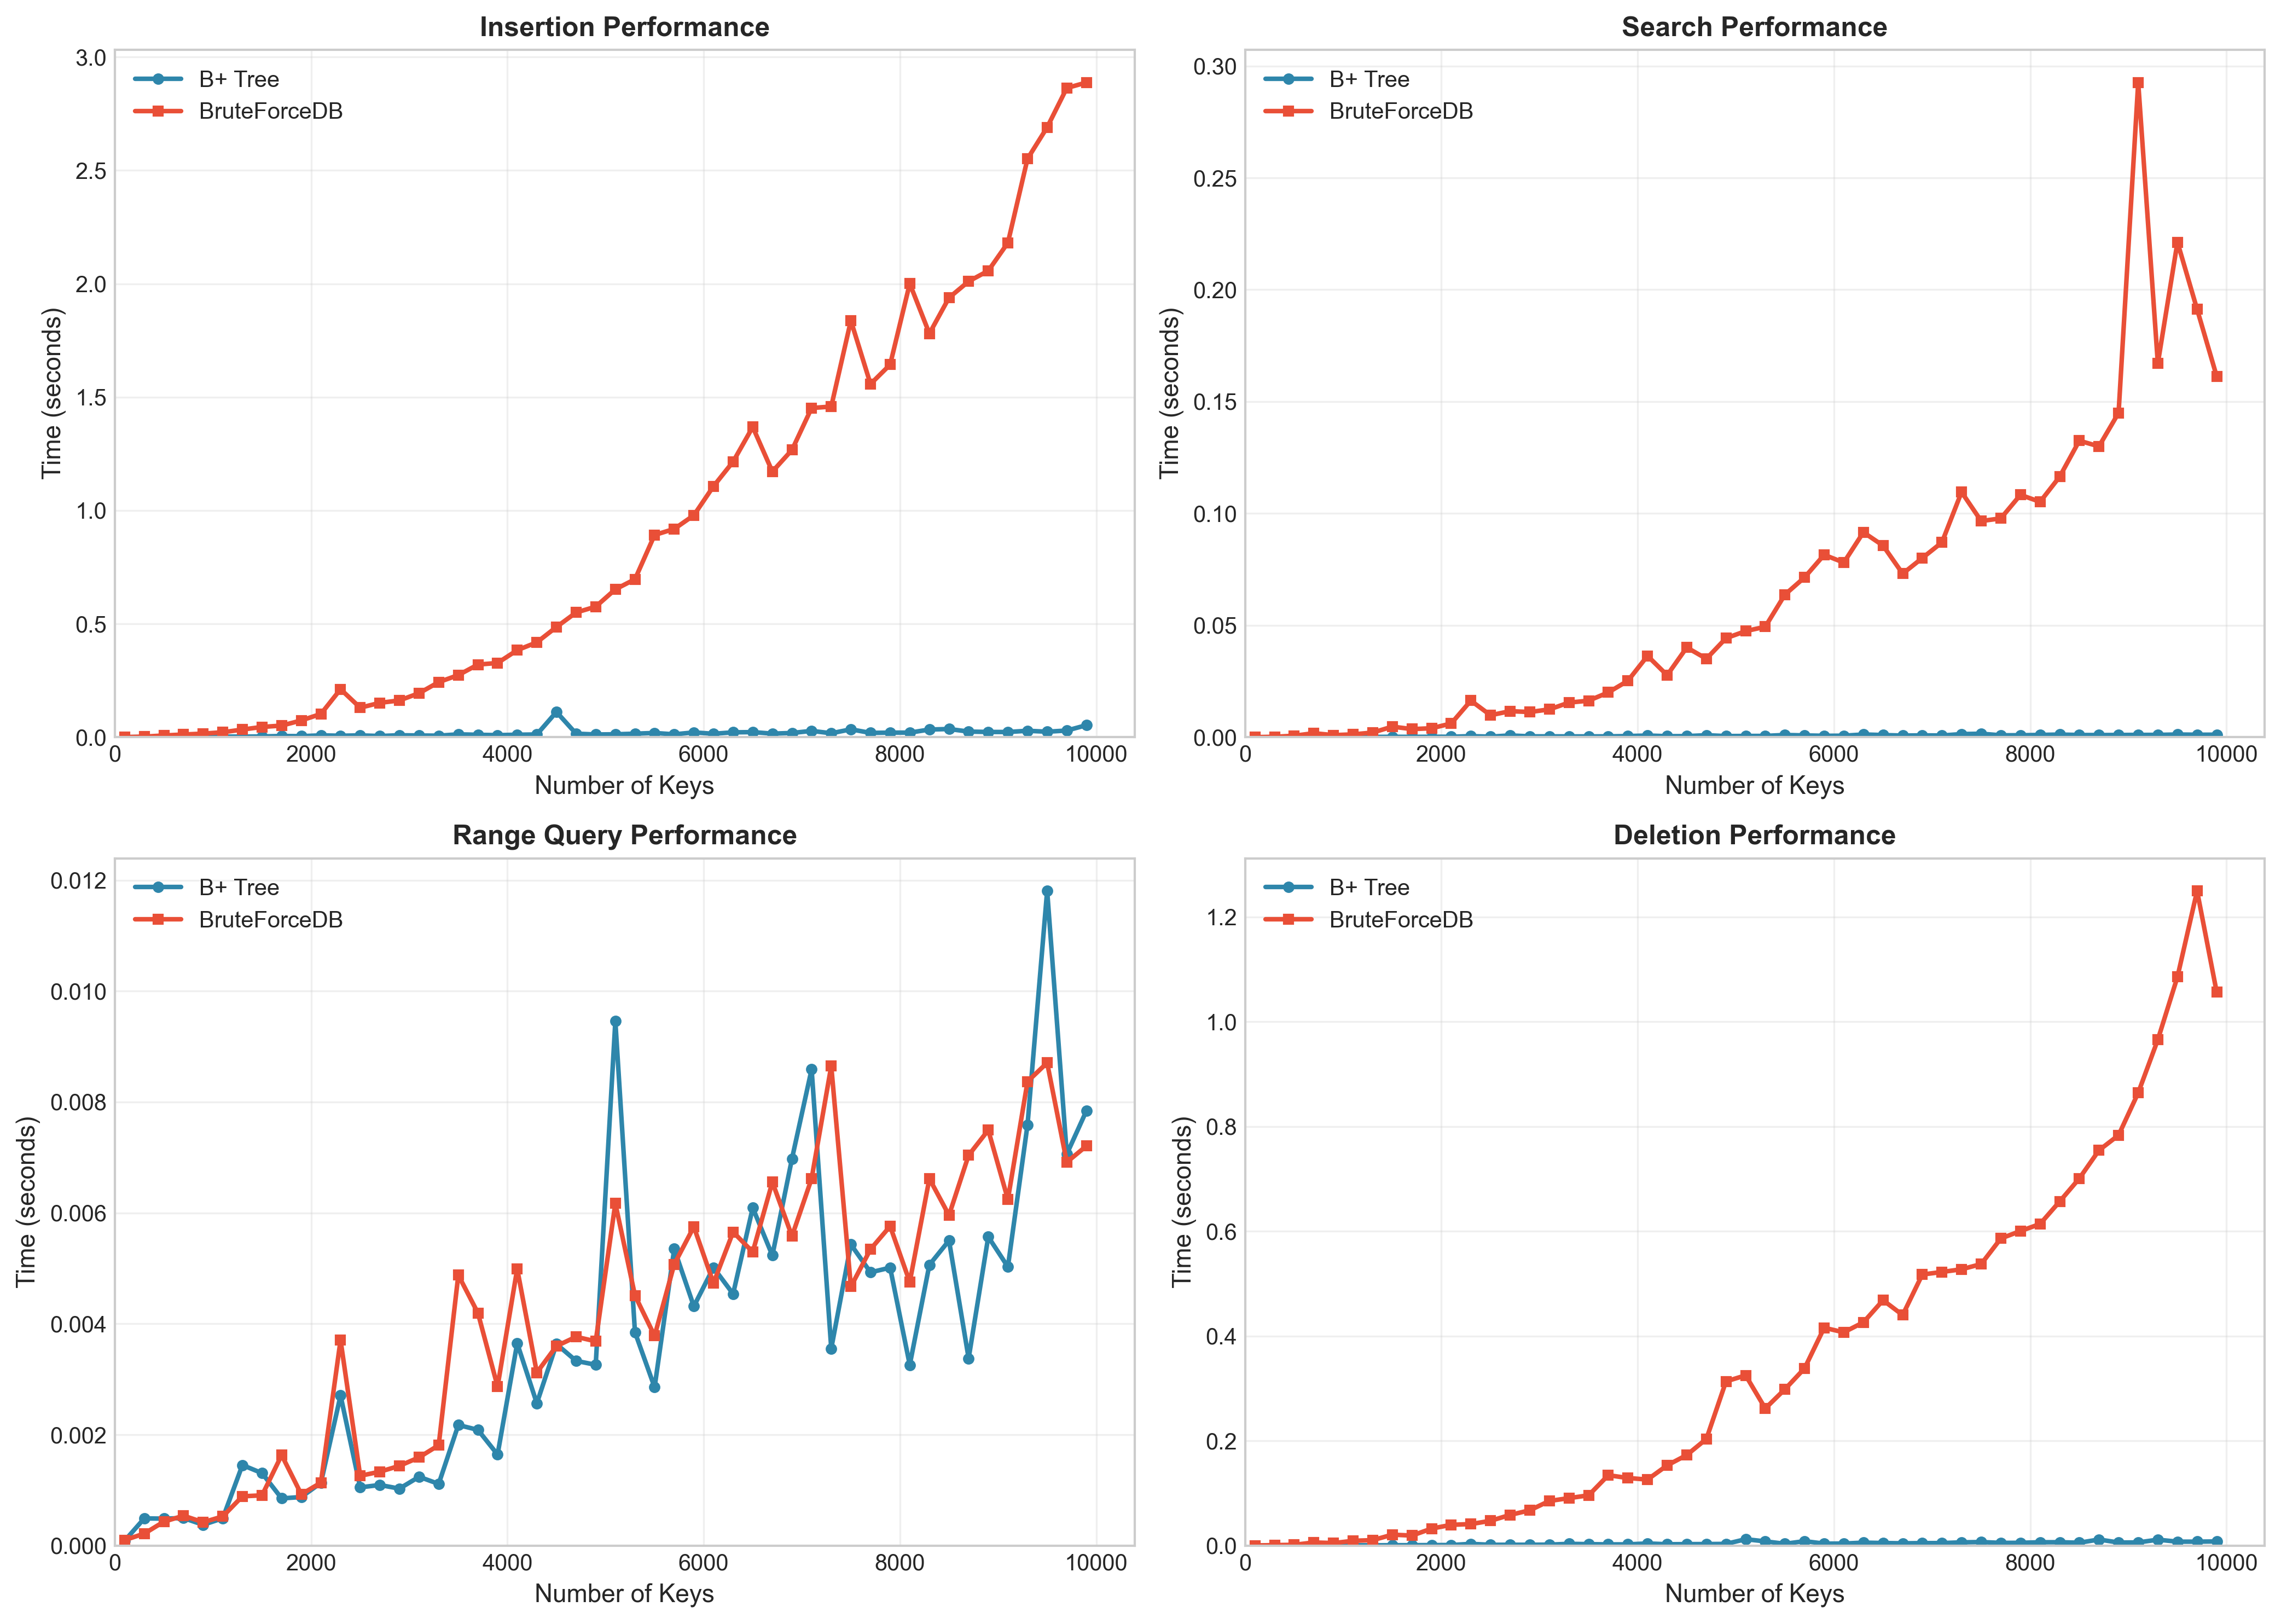
\includegraphics[width=0.95\textwidth]{visualizations/benchmark_plots/performance_comparison.png}
    \caption{Combined operation-wise runtime comparison.}
\end{figure}

\begin{figure}[H]
    \centering
    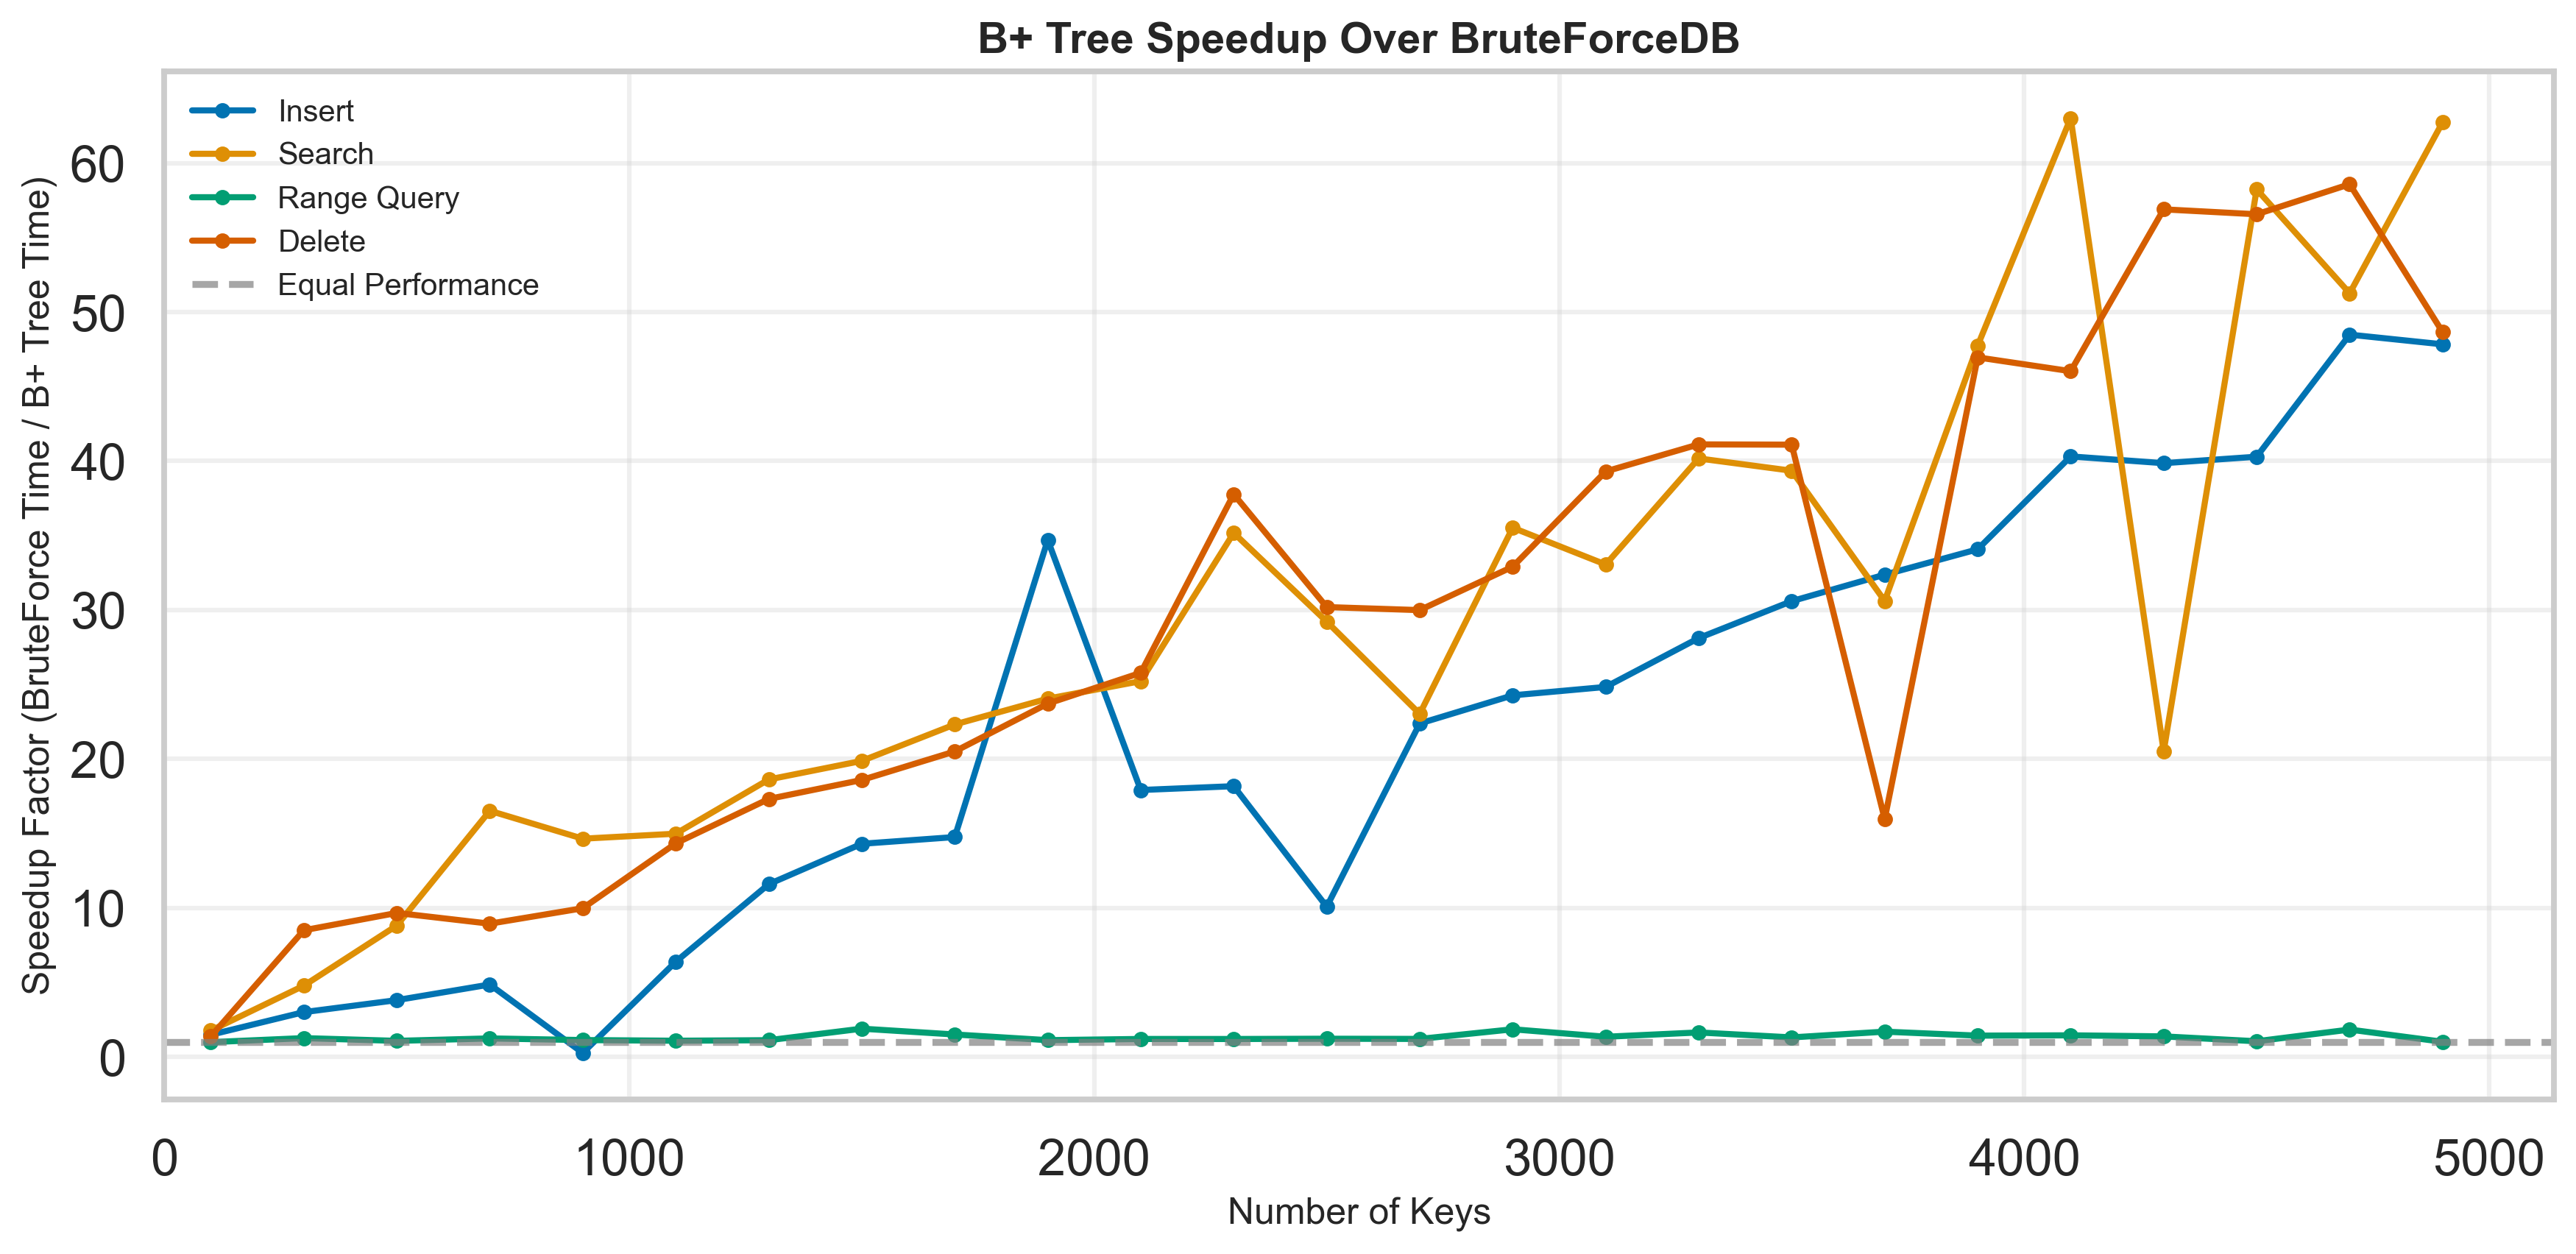
\includegraphics[width=0.85\textwidth]{visualizations/benchmark_plots/speedup_comparison.png}
    \caption{Speedup ratio (BruteForce time / B+ Tree time) across operation types.}
\end{figure}

\section{Visualisation}
The visualization outputs are used as structural correctness checks, not only as presentation artifacts. In particular, Section 3.2 of the notebook demonstrates staged structural evolution of the same tree under controlled insert and delete sequences.

These visual outputs are important because they provide direct evidence that balancing logic is functioning correctly under growth and shrinkage. In other words, the diagrams validate not just output correctness, but also \textbf{structural invariants} of the index.

\subsection{Stage-wise Tree Evolution (from Section 3.2 Notebook)}
\begin{figure}[H]
    \centering
    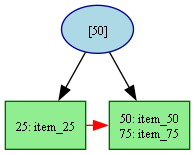
\includegraphics[width=0.68\textwidth]{visualizations/tree_outputs/stage2_initial.png}
    \caption{Stage 2: Tree after initial insertions [50, 25, 75].}
\end{figure}
\textbf{Explanation:} The tree remains shallow with a minimal internal routing structure; no deep split propagation is required at this stage.

\begin{figure}[H]
    \centering
    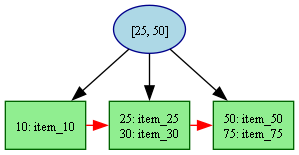
\includegraphics[width=0.68\textwidth]{visualizations/tree_outputs/stage3_after_split.png}
    \caption{Stage 3: after inserting [10, 30], first visible split behavior.}
\end{figure}
\textbf{Explanation:} A leaf overflow triggers split and separator promotion, establishing clearer internal partitioning.

\begin{figure}[H]
    \centering
    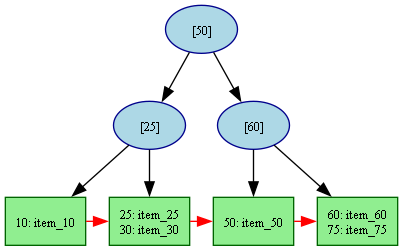
\includegraphics[width=0.68\textwidth]{visualizations/tree_outputs/stage4_after_split.png}
    \caption{Stage 4: after additional insertion (60), further redistribution.}
\end{figure}
\textbf{Explanation:} Local balancing preserves sorted routing while preventing skew; the shape adjusts without violating occupancy constraints.

\begin{figure}[H]
    \centering
    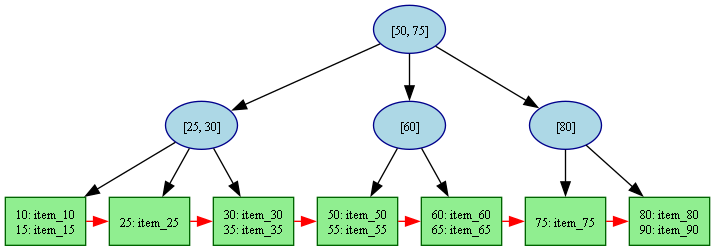
\includegraphics[width=0.74\textwidth]{visualizations/tree_outputs/stage5_larger.png}
    \caption{Stage 5: larger tree after additional insert workload.}
\end{figure}
\textbf{Explanation:} Height and fan-out increase in a controlled manner; all leaves remain at equal depth, preserving B+ Tree balance.

\begin{figure}[H]
    \centering
    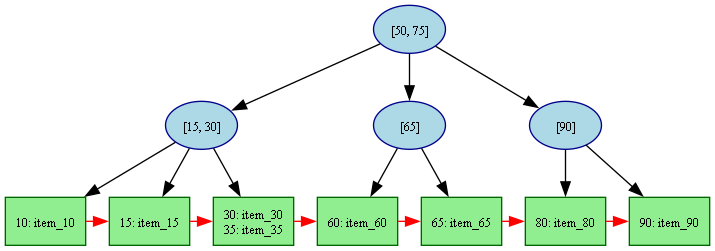
\includegraphics[width=0.74\textwidth]{visualizations/tree_outputs/stage6_after_delete.png}
    \caption{Stage 6: structure after deletion sequence and rebalancing.}
\end{figure}
\textbf{Explanation:} Delete-induced underflow is corrected through borrow/merge paths; the final shape remains valid and query-ready.

Taken together, the stage-wise sequence demonstrates stable structural behavior from initialization to split-heavy growth and then to deletion-driven rebalancing. This complements runtime benchmarking by confirming that performance is achieved without violating B+ Tree rules.

\section{Conclusion}
\subsection{Project Summary}
The Module A implementation demonstrates that B+ Tree indexing is a strong fit for Campus Trading workloads, particularly for mixed point-lookup and range-filter operations. By integrating balanced routing, linked-leaf traversal, and schema-aware table abstractions, the project delivers both algorithmic efficiency and practical usability.

\subsection{Challenges Faced}
The main implementation challenges were maintaining correct split propagation with parent pointer consistency, handling underflow robustly during deletion, and preserving leaf links during structural changes. These concerns were central to keeping the tree both valid and efficient under mixed CRUD workloads.

\subsection{Future Improvements}
Future work can focus on bulk loading for large sorted datasets, disk-backed persistence with page management, and concurrency control for multi-user scenarios. Additional optimization opportunities include caching frequently accessed nodes and applying key-compression strategies to reduce memory footprint.

\section{Work Distribution}
To ensure fairness and accountability, work was distributed \textbf{equally} across all five team members. Each member contributed approximately \textbf{20\%} of total effort with balanced involvement in design, implementation, testing, documentation, and review.

\begin{table}[H]
\centering
\caption{Equal Work Distribution Across Team Members}
\begin{tabular}{@{}lll@{}}
\toprule
Member & Primary Responsibility Set & Contribution \\
\midrule
Jinil Patel & B+ Tree core logic, split/merge validation, code review & 20\% \\
Hitesh Kumar & Node abstractions, invariants, delete-path testing & 20\% \\
Bhavik Patel & Benchmark framework, plots, performance interpretation & 20\% \\
Pranav Patil & Table/DB manager integration, workflow demonstrations & 20\% \\
Sibtain & Visualization pipeline, report writing, final consolidation & 20\% \\
\bottomrule
\end{tabular}
\end{table}

In addition to primary responsibility areas, all members participated in cross-review and validation of notebook outputs and report sections.

\end{document}
